\documentclass{report}

% set font encoding for PDFLaTeX, XeLaTeX, or LuaTeX
\usepackage{ifxetex,ifluatex}

\if\ifxetex T\else\ifluatex T\else F\fi\fi T%
  \usepackage{fontspec}
\else
  \usepackage[T1]{fontenc}
  \usepackage[utf8]{inputenc}
  \usepackage{lmodern}
\fi

\usepackage{amsmath}
\usepackage{amssymb}
\usepackage{amsthm}
\usepackage{bm}
\usepackage{bbm}
\usepackage{mathtools}
\usepackage{physics}

\usepackage{enumitem}
\usepackage{multicol}
\usepackage{graphicx}
\usepackage[dvipsnames]{xcolor}

\usepackage{hyperref}
\hypersetup{colorlinks=true,}
\usepackage[parfill]{parskip}
\usepackage{lipsum}
\usepackage[export]{adjustbox}
\usepackage{listings}

\usepackage{xparse} 
\usepackage{subfig} 
\usepackage{xparse} 
\usepackage{float}

\usepackage{biblatex} 

%%%%%This is an image table command, can likely be deleted
\newcommand{\subf}[2]{

%
{\small 
\begin{tabular}
  [t]{@{}c@{}} #1\ 
  \#2 
\end{tabular}
}

%
} 

\makeatletter
\renewcommand*\env@matrix[1][c]{\hskip -\arraycolsep
  \let\@ifnextchar\new@ifnextchar
  \array{*\c@MaxMatrixCols #1}}
\makeatother
%%%%%% Tensor Product
\NewDocumentCommand{\tens}{e{_^}}{ 
\mathbin{\mathop{\otimes}\displaylimits \IfValueT{#1}{_{#1}} \IfValueT{#2}{^{#2}} }}
%%%%%% Add \R Reals
\newcommand{\R}{\mathbb{R}} 
\newcommand{\N}{\mathbb{N}} 
\newcommand{\Z}{\mathbb{Z}} 
%%%%%% Missing citation warn
\newcommand{\CITEMISSING}{\colorbox{BurntOrange}{CITE ME}}
%%%%%% Add \theorem float
\newtheorem{theorem}{Theorem}
%%%%%% Add \definition float
\theoremstyle{definition} 
\newtheorem{definition}{Definition}[section]
%%%%%%%%%%%%%%%%%%%%%%%%%%%%%%%%%%%%%%%%%%%%%%%%%%%%%%%%%%%%%%%%%%%%%%%%%%%%%%%%%%%%%%%%%%%%%%%%%%%%%%%%%%%%%%%%%%%%%%%%%%
%%%%%Uncomment to add citation library 
\bibliography{lib} 
\title{Notes}
\author{David Helekal}

\begin{document}
\maketitle
\newpage
\tableofcontents
\newpage
%%%%%%%%%%%%%%%%%%%%%%%%%%%%%%%%%%%%%%%%%%%%%%%%%%%%%%%%%%%%
%%%%%%%%%%%%%%%%%%%%%%%%%%%%%%%%%%%%%%%%%%%%%%%%%%%%%%%%%%%%
%%%%%%%%%%%%%%%%%%%%%%%%%%%%%%%%%%%%%%%%%%%%%%%%%%%%%%%%%%%%
%%%%%%%%%%%%%%%%%%%%%%%%%%%%%%%%%%%%%%%%%%%%%%%%%%%%%%%%%%%%
\chapter{Questions}
\begin{itemize}
  \item Multi+ The second term in equation \ref{eq:multirate} (i.e. what's the bifurcation rate in the forward process) is likely not correct. Clearly this is inversely proportional to the $Neg$ of the lineage going extinct (or being birthed in the forward process), however presumably it should also be proportional to the $Neg$ of the parent lineage? The reasoning being the larger the population size of the parent lineage the likelier it is for a bifurcation event to occur.
  \item Note: there are mistakes in section \ref{section:multi}. The combination numbers need to be taken per subtree, and the bifurcation likelihood is just first iteration and needs further consideration.
\end{itemize}
%%%%%%%%%%%%%%%%%%%%%%%%%%%%%%%%%%%%%%%%%%%%%%%%%%%%%%%%%%%%
%%%%%%%%%%%%%%%%%%%%%%%%%%%%%%%%%%%%%%%%%%%%%%%%%%%%%%%%%%%%
%%%%%%%%%%%%%%%%%%%%%%%%%%%%%%%%%%%%%%%%%%%%%%%%%%%%%%%%%%%%
%%%%%%%%%%%%%%%%%%%%%%%%%%%%%%%%%%%%%%%%%%%%%%%%%%%%%%%%%%%%
\chapter{Methods}
\section{Coalescent Preliminaries}
The coalescent is a CTMC defined on the set $\{1 ... n\}$, parametrised via the coalescent rate, in our case $1/Neg(t)$, where $g$ is a scale parameter and $Neg(t)$ the effective population size at time $t$. Define $\alpha = Neg$
The transition rates of the coalescent process are given by 
\begin{gather*}
\lambda(j, j-1) = \binom{j}{2}\cdot\frac{1}{\alpha(t)}
\end{gather*}
The waiting times in the homogenous case are exponentially distributed
\begin{gather*}
P[W_j \leq s] = 1-\exp(-s\frac{\binom{j}{2}}{\alpha(t)})
\end{gather*}
Furthermore, the waiting times for individual coalescent events, conditioned on being less than the time between two consecutive sampling events $\Delta t$ are distributed as follows
\begin{gather}\label{eq:conditional}
P[W_j \leq s\mid W_j \leq \Delta t ] = \frac{P[W_j \leq s]}{P[W_j \leq \Delta t]} \quad\forall s \leq \Delta t
\end{gather}
In the inhomogenous case, the waiting times can be derived as follows:
For an inhomogenous CTMC, let $E_j(t)$ be the total exit rate from state $j$ at time $t$.
By the markov property individual exit events from a given state only depend on the state and given time, i.e. they form a time-inhomogenous poisson process.
As such the probability of no events in an interval $[t,t+s]\quad s\in \R^+$ is 
\begin{gather}
\exp(-\int_t^{t+s}E_j(\tau)d\tau) = \exp(-\int_0^{s}E_j(t+\tau)d\tau)
\end{gather}
The waiting times are defined as
\begin{gather}
W_j(t) = \inf\{s:X(t+s)\neq j \mid X(t) = j\}
\end{gather}
As such
\begin{gather}
W_j(t) > s \Rightarrow \forall \tau\in[t, t+s]\quad X(\tau) = j
\end{gather}
Furthermore the above relation holds iff no exit event have occured in the time interval $[t,t+s]$. As such:
\begin{align*}
&P[W_j(t) > s] = P[\text{no exit events in }[t,t+s]] = \exp(-\int_0^{s}E_j(t+\tau)d\tau)\\
&P[W_j(t) < s] = 1 - \exp(-\int_0^{s}E_j(t+\tau)d\tau)
\end{align*}
In the case of phylodynamic coalescent this becomes
\begin{gather}
P[W_j(t) \leq s] = 1 - \exp(-\int_0^{s}\frac{\binom{j}{2}}{\alpha(t+\tau)}d\tau)
\end{gather}
Note, the waiting times are still memoryless:
\begin{gather}
P\left[W_j(t) > s+u\mid W_j(t)>s \right] = P\left[W_j(t) > s+u\mid X(s)=j\right]
\end{gather}
By markov property
\begin{gather}
P\left[W_j(t) > s+u\mid X(s)=j\right] = P\left[W_j(t+s) > u\right]
\end{gather}
%%%%%%%%%%%%%%%%%%%%%%%%%%%%%%%%%%%%%%%%%%%%%%%%%%%%%%%%%%%%
%%%%%%%%%%%%%%%%%%%%%%%%%%%%%%%%%%%%%%%%%%%%%%%%%%%%%%%%%%%%
%%%%%%%%%%%%%%%%%%%%%%%%%%%%%%%%%%%%%%%%%%%%%%%%%%%%%%%%%%%%
%%%%%%%%%%%%%%%%%%%%%%%%%%%%%%%%%%%%%%%%%%%%%%%%%%%%%%%%%%%%
\subsection{Homogenous case}
The simulation of the coalescent process conditioned on sampling times follows a modified gillespie scheme. In order to facilitate the computation of the likelihoods of the individual simulated trees, it is preferred to avoid rejection sampling. As such we require sampling the conditional likelihood \ref{eq:conditional}. This is achieved by inverse transform sampling.
Let:
\begin{gather}\label{eq:cond_timedep}
\begin{aligned}
  u\sim& U([0,1])\\
  T(u) : P[T(u)\leq s] &= \frac{P[T(u) \leq s]}{P[T(u) \leq \Delta t]} \quad\forall s \leq \Delta t
\end{aligned}
\end{gather}
Where $T(u)$ is assumed to be monotone increasing and invertible.
\begin{align*}
  &&P[T(u)\leq s] &= P[u\leq T^{-1}(s)]\\
  &\Rightarrow& P[u\leq T^{-1}(s)] &= \frac{\int_0^s\lambda\exp(-\lambda t)dt}{\int_0^{\Delta t}\lambda\exp(-\lambda t)dt}\\
  &\Rightarrow& T^{-1}(s) &= \frac{1-\exp(-\lambda s)}{1-\exp(-\lambda \Delta t)}
\end{align*}
Defining $y\triangleq T^{-1}(s)$, we obtain the transform:
\begin{gather}
T(y) = \frac{-1}{\lambda}\log[1-y(1-\exp(-\lambda\Delta t))]
\end{gather}
The corresponding pdf evaluated at $u$ is
\begin{gather}
f_{\mathbf{T}(u)}(T(u)) = \lambda \left(\frac{1}{1-\exp(\lambda\Delta t)}-u\right)
\end{gather}
\newpage
\begin{figure}[h]
  \centering
    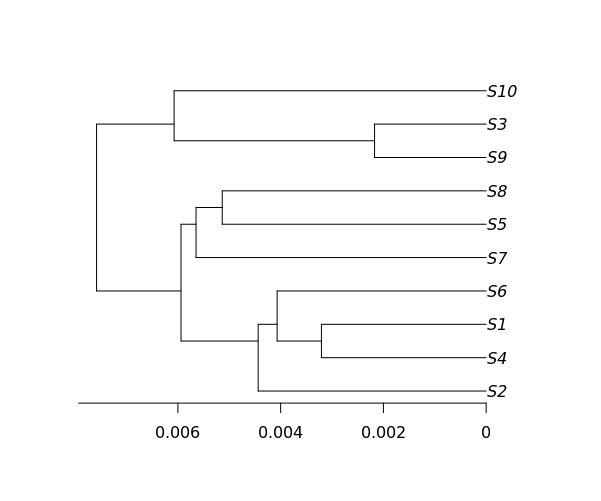
\includegraphics[width=0.5\textwidth]{plots/Coalescent_Example.png}
    \caption{An example simulated coalescent tree}
\end{figure}
%%%%%%%%%%%%%%%%%%%%%%%%%%%%%%%%%%%%%%%%%%%%%%%%%%%%%%%%%%%%
%%%%%%%%%%%%%%%%%%%%%%%%%%%%%%%%%%%%%%%%%%%%%%%%%%%%%%%%%%%%
%%%%%%%%%%%%%%%%%%%%%%%%%%%%%%%%%%%%%%%%%%%%%%%%%%%%%%%%%%%%
%%%%%%%%%%%%%%%%%%%%%%%%%%%%%%%%%%%%%%%%%%%%%%%%%%%%%%%%%%%%
\begin{lstlisting}
f <- (sampling_times, Ne): //Sampling times in descending order
  extant_lineages <- 1
  future_lineages <- length(sampling_times)-1
  t <- sampling_times[1]
  idx <- 1
  log_lh <- 0

  while extant_lineages > 1 or future_lineages > 0:
    if extant_lineages < 2:
      idx++
      t <- sampling_times[idx]
      extant_lineages++
      future_lineages--
    else:
      delta_t <- t-sampling_times[idx+1]
      rate <- binom(extant_lineages,2)/Ne

      p_coal <- 1-exp(-rate*delta_t)
      r_c ~ U[0,1] 

      if r_c < p_coal:

        log_lh += log(p_coal)

        coalesce_lineages
        extant_lineages--

        r_w ~ U[0,1]
        w_t <- (-1/rate)*log(1-r_w*(1-exp(-rate*delta_t)))
        t <- t+w_t

        cond_lh <- rate*(1/(1-exp(-rate*delta_t)) - r_w)
        log_lh += log(cond_lh)

      else:
        log_lh += log(1-p_coal)
        idx++
        t <- sampling_times[idx]
        extant_lineages++
        future_lineages--

    return: coalescent_times, log_lh
\end{lstlisting}
%%%%%%%%%%%%%%%%%%%%%%%%%%%%%%%%%%%%%%%%%%%%%%%%%%%%%%%%%%%%
%%%%%%%%%%%%%%%%%%%%%%%%%%%%%%%%%%%%%%%%%%%%%%%%%%%%%%%%%%%%
%%%%%%%%%%%%%%%%%%%%%%%%%%%%%%%%%%%%%%%%%%%%%%%%%%%%%%%%%%%%
%%%%%%%%%%%%%%%%%%%%%%%%%%%%%%%%%%%%%%%%%%%%%%%%%%%%%%%%%%%%
\subsection{Inhomogenous Case}
In the inhomogenous case, the scheme is similar, with the key difference that the sampling times now follow a much more complex distribution. We proceed with a modified conditional sampling scheme as in \ref{eq:cond_timedep}. To obtain draws $w_j(t)$, draws from standard exponential $w_j$ are rescaled, akin to algorithm described in \cite{hein_gene_2004} Pg 98.
%%%%%%%%%%%%%%%%%%%%%%%%%%%%%%%%%%%%%%%%%%%%%%%%%%%%%%%%%%%%
%%%%%%%%%%%%%%%%%%%%%%%%%%%%%%%%%%%%%%%%%%%%%%%%%%%%%%%%%%%%
%%%%%%%%%%%%%%%%%%%%%%%%%%%%%%%%%%%%%%%%%%%%%%%%%%%%%%%%%%%%
%%%%%%%%%%%%%%%%%%%%%%%%%%%%%%%%%%%%%%%%%%%%%%%%%%%%%%%%%%%%
\subsubsection{Waiting times distribution}
Consider the time interval $[t_i, s_i]$ with $s_j = min\left\{s\in S : s>t_i\right\}$. Define $\Delta t_i \triangleq s_i-t_i$.
The probability that no coalescent events happens within this interval is 
\begin{gather*}
  P[W_j(t_i) > \Delta t_i] = \exp(-\int_0^{\Delta t_i}\frac{\binom{j}{2}}{\alpha(t+\tau)}d\tau)
\end{gather*}
analogously, the probability of waiting times conditioned on that the waiting time is less than $\Delta t_i$ is:
\begin{gather}
  P[W_j(t_i) < s \mid W_j(t_i) < \Delta t_i] =\frac{1-\exp(-\int_0^{s}\frac{\binom{j}{2}}{\alpha(t+\tau)}d\tau)}{1-P[W_j(t_i) > \Delta t_i]}
\end{gather}
%%%%%%%%%%%%%%%%%%%%%%%%%%%%%%%%%%%%%%%%%%%%%%%%%%%%%%%%%%%%
%%%%%%%%%%%%%%%%%%%%%%%%%%%%%%%%%%%%%%%%%%%%%%%%%%%%%%%%%%%%
%%%%%%%%%%%%%%%%%%%%%%%%%%%%%%%%%%%%%%%%%%%%%%%%%%%%%%%%%%%%
%%%%%%%%%%%%%%%%%%%%%%%%%%%%%%%%%%%%%%%%%%%%%%%%%%%%%%%%%%%%
\subsubsection{Simulating}
In order to simulate $W_j(t_i)$ we proceed with an inverse transform sampling scheme, derived from the base samples $W_j$. 
First, assume $W_j$ are distributed according to 
\begin{gather}
  P[W_j < s \mid W_j < u] = \frac{1-\exp(-\frac{\binom{j}{2}}{\alpha})}{1-P[W_j>u]}
\end{gather}
Where $u$ is chosen such that
\begin{gather}
P[W_j>u] = P[W_j(t_i) > \Delta t_i]
\end{gather}
Then the function
\begin{gather}
F(W_j; t_i):\quad P[F(W_j;t_i) < s \mid W_j < u] = P[W_j(t_i) < s \mid W_j(t_i) < \Delta t_i] 
\end{gather}
Is given by the inverse with respect to $s$ of
\begin{gather}
G(s; t_i) = \int_0^s \frac{\alpha}{\alpha(t_i+\tau)}d\tau
\end{gather}
Which exists for any biologically sensible choice of $\alpha(t)$
\subsubsection{Likelihood}\label{subsection:likelihood}
Let $\left\{t_i\right\}_{i\in S\subset \N}$ denote the times of events in increasing order. Using notational convention from \cite{drummond_estimating_2002}, let $t_Y\triangleq \left\{t_i\right\}_{i\in Y}$ denote times of coalescent events and $t_I\triangleq \left\{t_i\right\}_{i\in I}$ denote times of sampling events, where $Y$, $I$ are disjoint partitions of the index set $S$ with the property that $S = Y\cup I$.
The likelihood of a particular genealogy is then given by:
\begin{gather}
\mathcal{L}\left(g\mid \alpha\right) 
= \prod_{i\in S\setminus 1}\left(\mathbbm{1}_Y(i)\frac{\binom{k_{i}}{2}}{\alpha(t_i)}+\mathbbm{1}_I(i)\right)
\exp(-\int_{t_{i-1}}^{t_i}\frac{\binom{k_{i}}{2}}{\alpha(\tau)}d\tau)
\end{gather}
The log-likelihood is:
\begin{gather}
\log\mathcal{L}\left(g\mid \alpha\right) 
= -\sum_{i\in S\setminus 1}{\int_{t_{i-1}}^{t_i}{\frac{\binom{k_{i}}{2}}{\alpha(\tau)d\tau}}} + \sum_{i\in Y}{\log\frac{\binom{k_{i}}{2}}{\alpha(t_i)}}
\end{gather}
%%%%%%%%%%%%%%%%%%%%%%%%%%%%%%%%%%%%%%%%%%%%%%%%%%%%%%%%%%%%
%%%%%%%%%%%%%%%%%%%%%%%%%%%%%%%%%%%%%%%%%%%%%%%%%%%%%%%%%%%%
%%%%%%%%%%%%%%%%%%%%%%%%%%%%%%%%%%%%%%%%%%%%%%%%%%%%%%%%%%%%
%%%%%%%%%%%%%%%%%%%%%%%%%%%%%%%%%%%%%%%%%%%%%%%%%%%%%%%%%%%%
\subsubsection{\textit{Skygrid} and other families of population functions}
\textit{Skygrid} is an approach introduced in \cite{gill_improving_2013}. It considers a family of time-dependent effective population size functions specified as follows. Let $T\subset\R$ be the interval under consideration in coalescent time. Consider an arbitrary population size function F:
\begin{gather}
  F:\quad T\subset\R \rightarrow \R^+
\end{gather}
Given a mutually disjoint family of time intervals $\left\{D_i\right\}_{i\in N}\subseteq T$, $D_j = [d_{j-1}, d_{j})$,  with $\bigcup\limits_{i\in N} D_i = T$, the \textit{skygrid} family of functions is then given by 
\begin{gather}
F_{skygrid}\triangleq\left\{\alpha\in F\mid\forall i\in N,\quad \forall t \in D_i,\quad \alpha(t) = c_i,\quad c_i\in\R^+\right\}
\end{gather}
This can be easily extended to any function $G$
\begin{gather}
 G(t)\triangleq\sum_{i\in N}{\mathbbm{1}_{D_i}(t)g_i(t)}
\end{gather}
Where $g_i(t)$ are arbitrary positive integrable functions.
Such formulation makes computation of likelihood straightforward.
\begin{gather}
\begin{aligned}
\log\mathcal{L}\left(g\mid G(t)\right) 
=& -\sum_{i\in S\setminus 1}{
\binom{k_i}{2}\sum_{j\in N}{\mathbbm{1}_{D_j}(t_{i-1})
\int_{t_{i-1}}^{\min\{d_j, t_i\}}{g^{-1}_j(\tau)d\tau}}}\\
&+\sum_{i\in Y}{\log\binom{k_i}{2}} - \sum_{i\in Y}{\log{\sum_{j\in N}{\mathbbm{1}_{D_j}(t_i)g_j(t_i)}}}
\end{aligned}
\end{gather}
%%%%%%%%%%%%%%%%%%%%%%%%%%%%%%%%%%%%%%%%%%%%%%%%%%%%%%%%%%%%
%%%%%%%%%%%%%%%%%%%%%%%%%%%%%%%%%%%%%%%%%%%%%%%%%%%%%%%%%%%%
%%%%%%%%%%%%%%%%%%%%%%%%%%%%%%%%%%%%%%%%%%%%%%%%%%%%%%%%%%%%
%%%%%%%%%%%%%%%%%%%%%%%%%%%%%%%%%%%%%%%%%%%%%%%%%%%%%%%%%%%%
\section{Inhomogenous Lineages and Outbreaks}\label{section:multi}
Suppose we sample genomes of a set of pathogenic bacterial samples. 
At an unknow point in time a particular strain acquires a mutation conferring it resistance to a widely used antibiotic. This increases the particular strains fitness and enables it to undergo a period of rapid growth leading to a clonal expansion. If we assume that this increase in fitness occurs in a short time span, the lineage of this strain will behave differently in the phylogenetic tree, having a coalescent rate corresponding to a rapidly expanding population, starting from a very small number of individuals\CITEMISSING. This problem of identifying hidden population structure has been proposed in \cite{volz_identification_nodate}, where a testing based approach was used to indentify structure in a phylogeny.\\

We seek a modification to the coalescent model that will allow for change points located on the branches of the phylogeny, marking the event when a particular lineage starts behaving according to a different population size function than its parent lineage.\\

In this model, coalescent nodes have an added colour property, and each colour coalesces according to a colour specific, time dependent case. Nodes of non-identical colour can coalesce iff at least one of them is the last remaining node of a given colour.
Different colours correspond to different lineages, each behaving under its own growth function.\\

Similar models, refered to as Structured Coalescent, adding colouring to vertices of phylogenies have been used in epidemiology to track outbreaks \cite{maio_scotti_2016}, or transmission chains \cite{didelot_genomic_2017}.
%%%%%%%%%%%%%%%%%%%%%%%%%%%%%%%%%%%%%%%%%%%%%%%%%%%%%%%%%%%%
%%%%%%%%%%%%%%%%%%%%%%%%%%%%%%%%%%%%%%%%%%%%%%%%%%%%%%%%%%%%
%%%%%%%%%%%%%%%%%%%%%%%%%%%%%%%%%%%%%%%%%%%%%%%%%%%%%%%%%%%%
%%%%%%%%%%%%%%%%%%%%%%%%%%%%%%%%%%%%%%%%%%%%%%%%%%%%%%%%%%%%
\subsection{Model}
A given genealogy $\mathbf{g}=(V_\mathbf{g}, E_\mathbf{g}, t_\mathbf{g})$ is an incomplete, empirical sample of the underlying process\CITEMISSING.\\
It consists of nodes $V_\mathbf{g}$, directed edges $E_\mathbf{g}$, and node labels $t_\mathbf{g}$ corresponding to event times.\\
As in section \ref{subsection:likelihood} $\mathbf{g}$ shall be indexed by an index set $S=1\leq i \leq N\subset \N$, with $Y\subset S$ corresponding to coalescent events and $I\subset S$ corresponding to sampling events.\\
For convenience, assume that all edges are in the forwards time direction, i.e.: 
\begin{gather*}
\forall k,l \in S: (k,l)\in E_\mathbf{g} \Rightarrow t_k<t_l
\end{gather*}
Furthermore, all event times are ordered in descending (backwards) time order, i.e.:
\begin{gather*}
\forall k,l \in S: k<l \Rightarrow t_k > t_l
\end{gather*}
Under the assumption that $\mathbf{g}$ is a genealogy of a given sample, with each edge in $E_\mathbf{g}$ there is an associated unobserved set of individuals descending from one another\CITEMISSING. At some point along an edge a node of one lineage will undergo colour change and change its type to that of another lineage.\\
We seek a model which enable us to investigate this proposed behaviour.
\begin{definition}[Multiple Lineage Coalescent]\label{def:model}
Given $M$ colours, $M$ population size functions $\mathbf{\alpha}\triangleq\{\alpha_j(t)\}_{1\leq j\leq M}$. Let $Y(t)$ be a CTMC with the state space:
\begin{gather}
  \Sigma = \left\{\mathbf{s}\in \Z_+: |\mathbf{s}|\geq1\right\}
\end{gather}
and the transition rates
\begin{gather}\label{eq:multirate}
\begin{align}
\mathbf{s}&\to\mathbf{s}-\mathbf{e_j} &\quad& \binom{s_j}{2}\alpha_j^{-1}(t)&\quad&1\leq j\leq M\\
\mathbf{s}&\to\mathbf{s}-\mathbf{e_j}+\mathbf{e_k}&\quad& \delta_{1,j}s_k&\quad&1\leq j,k\leq M
\end{align}
\end{gather}
\end{definition}
The interpretation of this model in backwards (coalescent) time is that each node corresponds to a single specific lineage (colour). Nodes of the same lineage coalesce at i.i.d rates, according to a lineage specific growth functions, until reaching the MRCA of given lineage. The MRCA then changes type (colour) to that of a different lineage. \\
Under the hypothesis, along each of the edges from the parent of a lineage MRCA to the MRCA lies a point in time that characterises the time of divergence of the lineage, after which the lineage starts to undergo clonal expansion.

\subsection{Inference}
Assume that we have been given a genealogy as described in previous section. The number of individua lineages $M$, the effective population size functions $\mathbf{\alpha}$, the placement and divergence events in descending order $\Xi =\{\xi_i\}_{1\leq i\leq M}$, are unknown. In effect we seek to identify terms in the factorisation of the posterior:
\begin{gather}
\mathcal{L}(\mathbf{\alpha}, \Xi, M\mid\mathbf{g}) \propto 
\mathcal{L}(\mathbf{g}\mid \Xi, M, \mathbf{\alpha})\mathcal{L}(\mathbf{\alpha}\mid\Xi,M)\mathcal{L}(\Xi,M)
\end{gather}

\begin{definition}[Divergence Event] A divergence event $\xi$ associated with a lineage is a tuple:
\begin{gather}
\xi=\left(e', \tau\right)
\end{gather}
where $\tau$ denotes the time of the divergence event, and $e' = (v^{pa}, v^{MRCA})$ denotes the edge along which the divergence event happens, with $v^{MRCA}$ being the MRCA of the newly diverging lineage.
\end{definition}
In order to identify the likelihood $\mathcal{L}(\mathbf{g}\mid \Xi, M, \mathbf{\alpha})$, the genealogy needs to be first partitinioned into separate subtrees, each corresponding to an individual lineage.

\begin{definition}[Descendant Set]
\begin{gather}
\begin{aligned}
\mathcal{D}(i) &\triangleq \{j\in S\mid j \text{ is a descendant of } i\}
\end{aligned}
\end{gather} 
\end{definition}

\begin{definition}[Lineage Subtree]
A subtree $W(\xi_i)$ associated with a divergence event $\xi_i$ consists of all vertices, edges and times associated with a given lineage.
\begin{gather}
W(\xi_i) \triangleq \mathcal{D}(v^{pa}_i) \setminus \bigcup_{j<i}(\mathcal{D}(v^{pa}_j))
\end{gather} 
\end{definition}
As members of a lineage can only coalesce with one another, the coalescence rate is independent of other lineages, and the time of divergence has been given, the total likelihood is equal to the product of individual lineage specific likelihoods.\\
A final step before deriving lineage specific likelihoods is required, that is, the divergence times have to be included along with the times contained within the lineage subtree.\\

Denote the set of all divergence times associated with a Lineage Subtree $W(\xi_j)$ $\tau_{W(\xi_j)}$
\begin{gather*}
\tau_{W(\xi_j)} \triangleq \tau_i \in \xi_i : v^{pa}_i \in W(\xi_j), \quad \forall 1\leq i\leq M
\end{gather*}
Finally define the set of all times associated with a particular lineage
$T(\xi_j) = \tau_{W(\xi_j)}\cup t_{W(\xi_j)}$, indexed by set $S_{T(\xi_j)}=\{1 ... |T(\xi_j)|\}$ such that
\begin{gather*}
\forall t_k, t_l \in T(\xi_j),\quad k>l \Rightarrow t_k \geq t_l
\end{gather*}
Let $k_{i,\xi_j}$ denote the number of extant individuals corresponding to subtree lineage $\xi_j$ at during the time interval $[t_{i-1}, t_i]$.
The total likelihood is equal to:
\begin{gather}
\begin{aligned}
\mathcal{L}(\mathbf{g}\mid \Xi, M, \mathbf{\alpha}) &= \prod_{j=1}^{M}\mathcal{L}(T(\xi_j) \mid \alpha_j) \\
\mathcal{L}(T(\xi_j) \mid \alpha_j) &= \prod_{t_i\in T(\xi_j)}\left(\mathbbm{1}_{t_Y}(t_i) \frac{\binom{k_{i,\xi_j}}{2}}{\alpha(t_i)}+\mathbbm{1}_{t_I\cup\tau_{W(\xi_j)}}(t_i)\right)
\exp(-\int_{t_{i-1}}^{t_i}\frac{\binom{k_{i,j}}{2}}{\alpha(\tau)}d\tau)
\end{aligned}
\end{gather}
\subsection{Choice of Population Size Functions}
\subsubsection{SIS Model}
The dynamics of an immunity non-confering pathogen with the host population constant can be described by the SIS model\cite{keeling_introduction_2008}:
\begin{gather}
\frac{dI}{dt'} = (N-I)\beta I/N -\gamma I
\end{gather}
By defining $A=\beta-\gamma$ and $B=\beta/N$, we obtain the solution 
This equation admits a solution of the form:
\begin{gather}
I(t') = \frac{A}{B+(A/I_0-B)\exp(-t'A)}
\end{gather}
We assume $I_0$ = 1.
This can be rearranged and contrasted with standard logistic growth with carrying capacity equal to $A/B$ and growth rate equal to $A$: 
\begin{gather}
I(t') = \frac{A/B}{1+(A/B - 1)\exp(-t'A)}
\end{gather}
As our hypothesis posutlates that a divergence event is a new lineage being born and undergoing rapid growth, we require $\alpha(0) = 0$. Hence we take $\alpha(t') = I(t')-1$.\\
Finally in order to convert into population decline in coalescent time, perform the change of variables $-t'+T_{max} - T_{div} = \tau$, while also defining $K=A/B$:
\begin{gather}
\begin{aligned}
  \alpha(\tau) &= \frac{K}{1+(K - 1)\exp((\tau-T_{max}+T_{div})A)}-1\\
               &= \frac{(K-1)- (K - 1)\exp((\tau-T_{max}+T_{div})A)}{1+(K - 1)\exp((\tau-T_{max}+T_{div})A)}
\end{aligned}
\end{gather}
And
\begin{gather}
\begin{aligned}
&\alpha^{-1}(\tau) &=&  \frac{1+(K - 1)\exp((\tau-T_{max}+T_{div})A)}{(K-1)- (K - 1)\exp((\tau-T_{max}+T_{div})A)}\\
&\Rightarrow&& \frac{1}{(K-1)(1-\exp((\tau-T_{max}+T_{div})A))}\\
&&+& \frac{1}{\exp(-(\tau-T_{max}+T_{div})A)-1}
\end{aligned}
\end{gather}
As such:
\begin{gather}
\begin{aligned}
&\int_t^{t+s}{\alpha^{-1}(\tau)\,d\tau}&=& \left[\frac{-1}{(K-1)A}\log(\exp(-(\tau-T_{max}+T_{div})A)-1)\right]_t^{t+s}\\
&&+&\left[\frac{1}{A}\log(1-\exp((\tau-T_{max}+T_{div})A))\right]_t^{t+s}\\
&\Rightarrow&&\left[\frac{K-2}{(K-1)A}\log(\frac{1-\exp((\tau-T_{max}+T_{div})A)}{\exp(-(\tau-T_{max}+T_{div})A)-1})\right]_t^{t+s}
\end{aligned}
\end{gather}
Define $Q=\frac{K-2}{(K-1)A}$, $T = T_{max}+T_{div}$, expanding the integral:
\begin{gather}
\begin{aligned}
&Q\left[\log(\frac{1-\exp((t+s-T)A)}{\exp(-(t+s-T)A)-1})-\log(\frac{1-\exp((t-T)A)}{\exp(-(t-T)A)-1})\right]\\
=&Q\left[\log(\frac{(1-\exp((t+s-T)A))(\exp(-(t-T)A)-1)}{(\exp(-(t+s-T)A)-1)(1-\exp((t-T)A))})\right]\\
=&Q\left[\log(\frac{\exp(-(t-T)A) - \exp(sA) + \exp((t+s-T)A)) - 1 }{-\exp(-sA) + \exp((t-T)A) + \exp(-(t+s-T)A) - 1})\right]\\
=&Q\left[\log(\frac{\exp(sA)(\exp((t-T)A) - 1)+\exp(-(t-T)A)-1}{\exp(-sA)(\exp(-(t-T)A) - 1)+\exp((t-T)A)-1})\right]\\
=&Q\left[\log(\frac{\exp(sA)(\exp((t-T)A) - 1) - \exp(-(t-T)A)(\exp((t-T)A)-1)}{\exp(-sA)(\exp(-(t-T)A) - 1) - \exp((t-T)A)(\exp(-(t-T)A)-1)})\right]\\
=&Q\left[\log(\frac{(\exp((t-T)A)-1)(\exp(sA)-\exp(-(t-T)A))}{(\exp(-(t-T)A)-1)(\exp(-sA)-\exp((t-T)A))})\right]\\
=&Q\left[\log(\frac{(\exp((t-T)A)-1)}{\exp(-(t-T)A)-1})+\log(\frac{\exp(sA)-\exp(-(t-T)A)}{\exp(-sA)-\exp((t-T)A)})\right]
\end{aligned}
\end{gather}
Set $\rho=\frac{(\exp((t-T)A)-1)}{\exp(-(t-T)A)-1}$, $Y=\int_t^{t+s}{\alpha^{-1}(\tau)\,d\tau}$, $\phi=-\exp(Y/Q-\log(\rho)), \psi = \exp((t-T)A))-\exp(-(t-T)A)$
\begin{gather}
\begin{aligned}
Y/Q - \log(\rho) &= \log(\frac{\exp(sA)-\exp(-(t-T)A)}{\exp(-sA)-\exp((t-T)A)})\\
\exp(Y/Q-\log(\rho)) &= \frac{\exp(sA)-\exp(-(t-T)A)}{\exp(-sA)-\exp((t-T)A)}\\
-\phi(\exp(-sA)-\exp((t-T)A)) &= \exp(sA)-\exp(-(t-T)A)\\
\exp(sA) + \psi + \phi(\exp(-sA) &= 0\\
\exp(2sA) + \psi\exp(sA) + \phi &= 0
\end{aligned}
\end{gather}
By defining $x=\exp(sA)$, this becomes a quadratic equation. yielding the solution:
\begin{gather}
\begin{aligned}
&&x_{1,2} &= \frac{-\psi \pm \sqrt{\psi^2 - 4\phi}}{2}\\
&\Rightarrow& s &= \frac{1}{A}\log(x)
\end{aligned}
\end{gather}

\subsubsection{Gompertz Curve}
\subsection{Priors}
As a prior for change points $\mathcal{L}(\Xi,M)$ a Poisson Point Process is used. Denote by $B$ the total branch length of the genealogy. Then
\begin{gather}
M\sim\frac{(\lambda B)^M}{M!}\exp(-\lambda B)
\end{gather}
and 
\subsubsection{MCMC}
Due to the variable nature of the dimensionality of the parameter space, it will be necessary to use Reversible Jump MCMC (rjMCMC) \cite{fan_reversible_2010,green_reversible_1995}.
%%%%%%%%%%%%%%%%%%%%%%%%%%%%%%%%%%%%%%%%%%%%%%%%%%%%%%%%%%%%
%%%%%%%%%%%%%%%%%%%%%%%%%%%%%%%%%%%%%%%%%%%%%%%%%%%%%%%%%%%%
%%%%%%%%%%%%%%%%%%%%%%%%%%%%%%%%%%%%%%%%%%%%%%%%%%%%%%%%%%%%
%%%%%%%%%%%%%%%%%%%%%%%%%%%%%%%%%%%%%%%%%%%%%%%%%%%%%%%%%%%%
\chapter{Results}
\section{Simulations}
\subsection{Exponetial Growth}
An example of a population under exponential growth, $\alpha(t) = N*\exp(-\lambda t)$ consisting of 100 sampling events between 0 and 10 years before present has been simulated with a rate parameter $\lambda$ and final size parameter $N$ drawn from a uniform densities on intervals $[0.1, 10]$, and $[1,100]$ respectively.\\
A Metropolis-Hastings MCMC scheme was then used to infer the parameters $\lambda$ and $N$. A zero-centred laplace distribution with rate equal to one was chosen as the prior for $\lambda$, whereas for $N$ the exponential distribution with rate one was used.\\
One million iterations were used and the first One hundred thousand discarded as burn in time. To further validate the fit, both a maximum likelihood (MLE) and maximum \textit{a-posteriori} (MAP) estimates were computed and plotted against the posterior marginals inferred by the MCMC.
%%%%%%%%%%%%%%%%%%%%%%%%%%%%%%%%%%%%%%%%%%%%%%%%%%%%%%%%%%%%
%%%%%%%%%%%%%%%%%%%%%%%%%%%%%%%%%%%%%%%%%%%%%%%%%%%%%%%%%%%%
%%%%%%%%%%%%%%%%%%%%%%%%%%%%%%%%%%%%%%%%%%%%%%%%%%%%%%%%%%%%
%%%%%%%%%%%%%%%%%%%%%%%%%%%%%%%%%%%%%%%%%%%%%%%%%%%%%%%%%%%%
\begin{figure}[H]
  \centering
  \subfloat[]{\label{trace:a}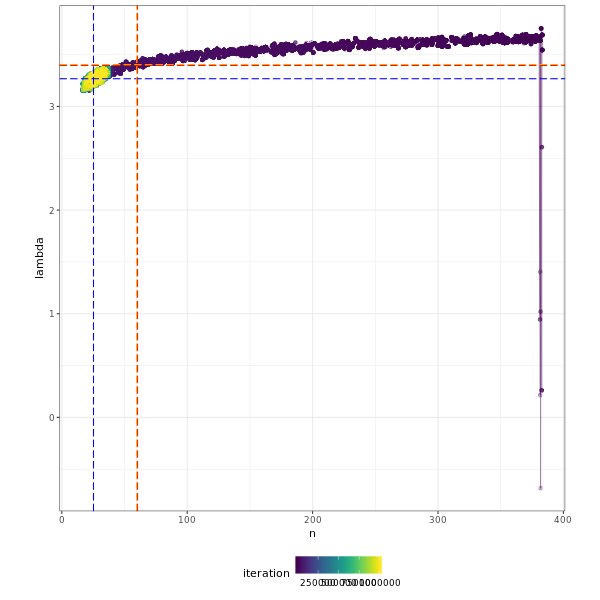
\includegraphics[scale=.25]{../R/trace}}
  \centering
  \subfloat[]{\label{trace:b}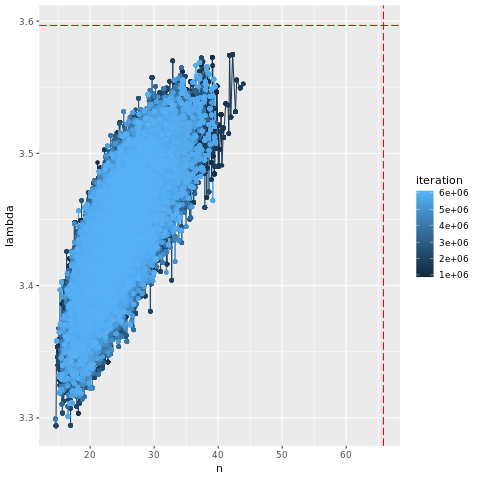
\includegraphics[scale=.25]{../R/trace_zoom}}
  \centering
  \caption{Trace plots for the markov chain. Red lines denote true parameter values. MLE marked by blue lines. MAP marked by orange lines. \ref{trace:a} Shows the entire trace of the chain. \ref{trace:b} Shows the trace with the first 100000 iterations discarded}
  \label{fig:trace}
\end{figure}
%%%%%%%%%%%%%%%%%%%%%%%%%%%%%%%%%%%%%%%%%%%%%%%%%%%%'%%%%%%%%
%%%%%%%%%%%%%%%%%%%%%%%%%%%%%%%%%%%%%%%%%%%%%%%%%%%%%%%%%%%%
%%%%%%%%%%%%%%%%%%%%%%%%%%%%%%%%%%%%%%%%%%%%%%%%%%%%%%%%%%%%
%%%%%%%%%%%%%%%%%%%%%%%%%%%%%%%%%%%%%%%%%%%%%%%%%%%%%%%%%%%%
\begin{figure}[H]
  \centering
  \subfloat[]{\label{hists:a}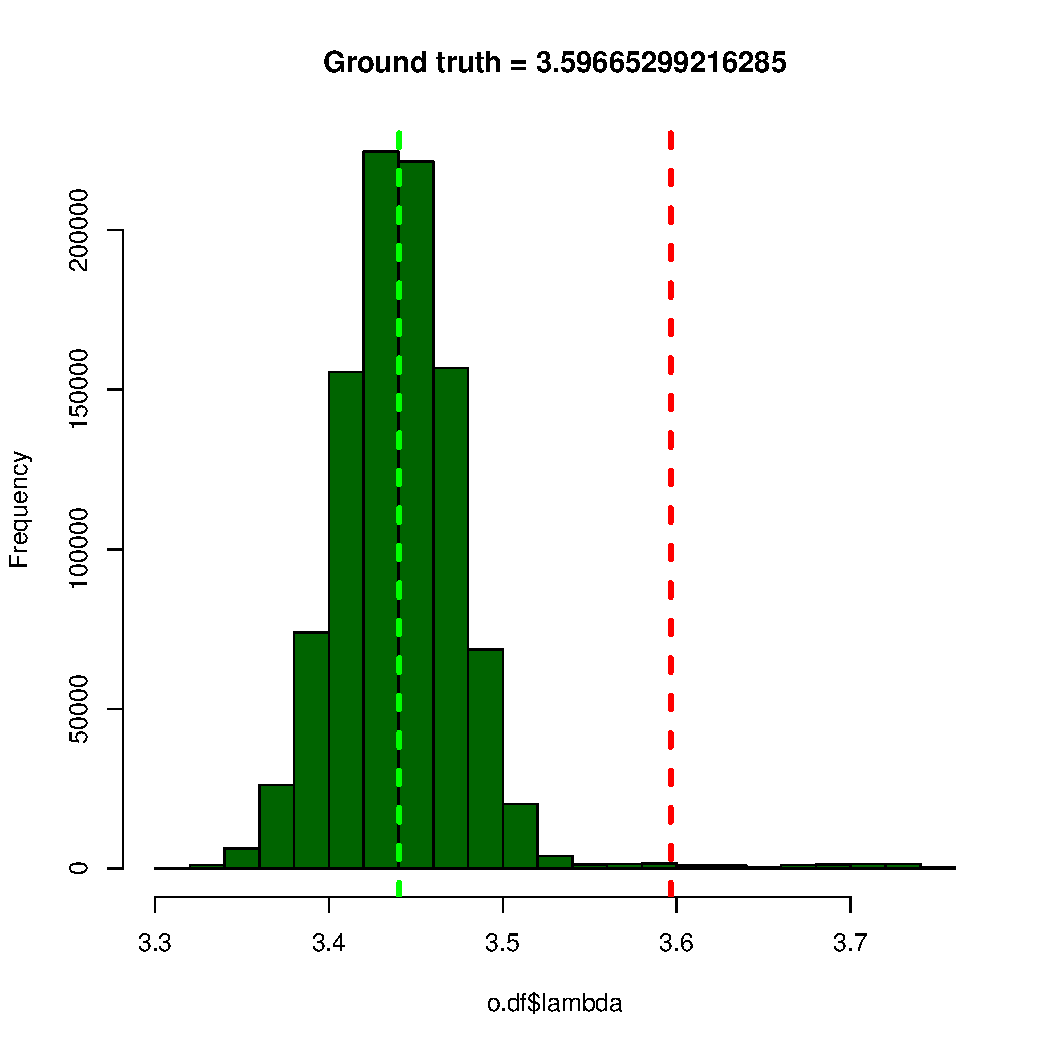
\includegraphics[scale=.4]{../R/lambdahist}}
  \centering
  \subfloat[]{\label{hists:b}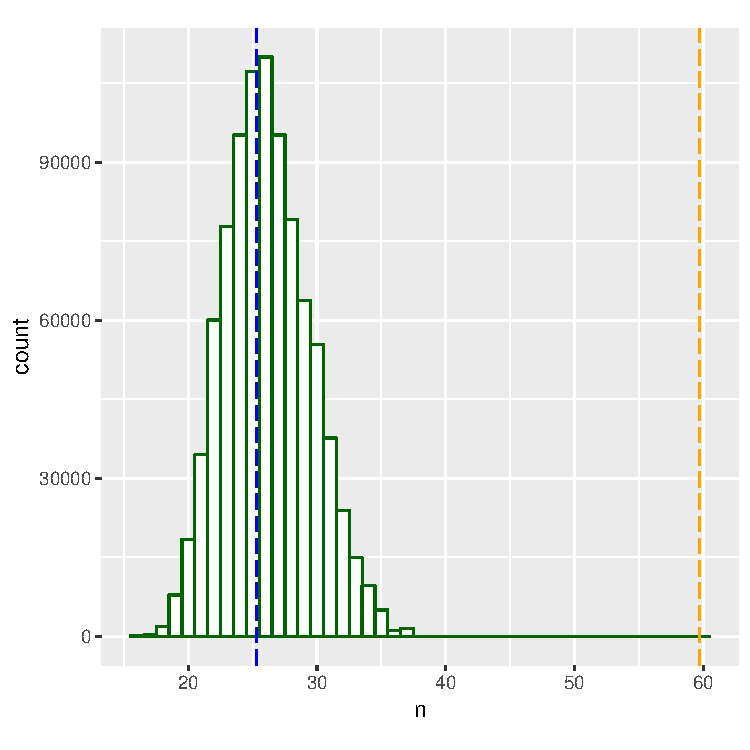
\includegraphics[scale=.4]{../R/nhist}}
  \centering
  \caption{Histograms of the posterior marginals. MLE marked by blue line. MAP marked by orange line. \ref{hists:a} $\lambda$ marginal \ref{hists:b} $N$ marginal}
  \label{fig:hists}
\end{figure}
\begin{figure}[H]
  \centering
    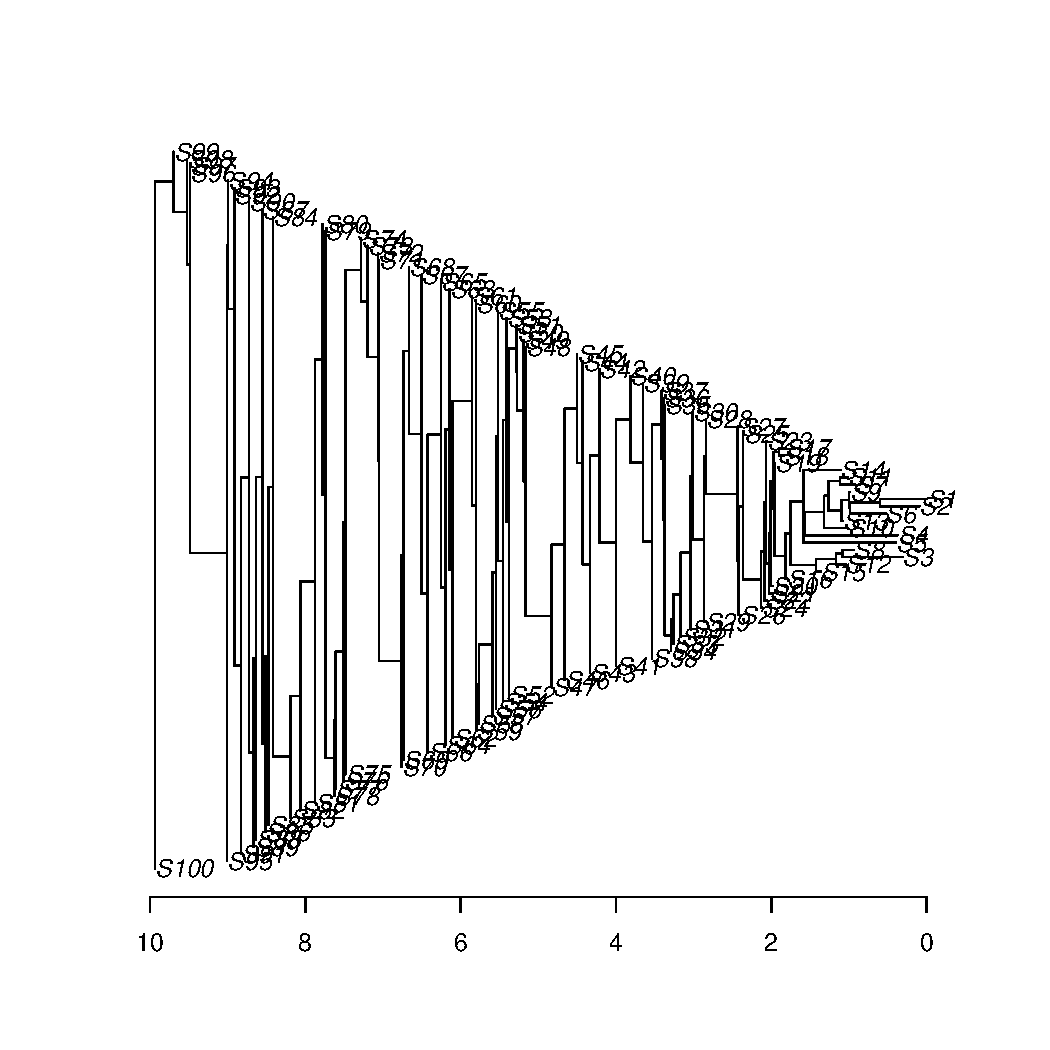
\includegraphics[width=0.5\textwidth]{../R/tree}
    \caption{The simulated genealogy used for this example.}
\end{figure}
%%%%%%%%%%%%%%%%%%%%%%%%%%%%%%%%%%%%%%%%%%%%%%%%%%%%%%%%%%%%
%%%%%%%%%%%%%%%%%%%%%%%%%%%%%%%%%%%%%%%%%%%%%%%%%%%%%%%%%%%%
%%%%%%%%%%%%%%%%%%%%%%%%%%%%%%%%%%%%%%%%%%%%%%%%%%%%%%%%%%%%
%%%%%%%%%%%%%%%%%%%%%%%%%%%%%%%%%%%%%%%%%%%%%%%%%%%%%%%%%%%%
\section{Previous Work}
A framework utilising sampling intensity in order to extract more information is proposed in \cite{parag_jointly_nodate}
%%%%%%%%%%%%%%%%%%%%%%%%%%%%%%%%%%%%%%%%%%%%%%%%%%%%%%%%%%%%
%%%%%%%%%%%%%%%%%%%%%%%%%%%%%%%%%%%%%%%%%%%%%%%%%%%%%%%%%%%%
%%%%%%%%%%%%%%%%%%%%%%%%%%%%%%%%%%%%%%%%%%%%%%%%%%%%%%%%%%%%
%%%%%%%%%%%%%%%%%%%%%%%%%%%%%%%%%%%%%%%%%%%%%%%%%%%%%%%%%%%%
\section{Bibliography}
\printbibliography
\end{document}
